
\begin{comment}
\begin{figure*}[!h]
\begin{center}
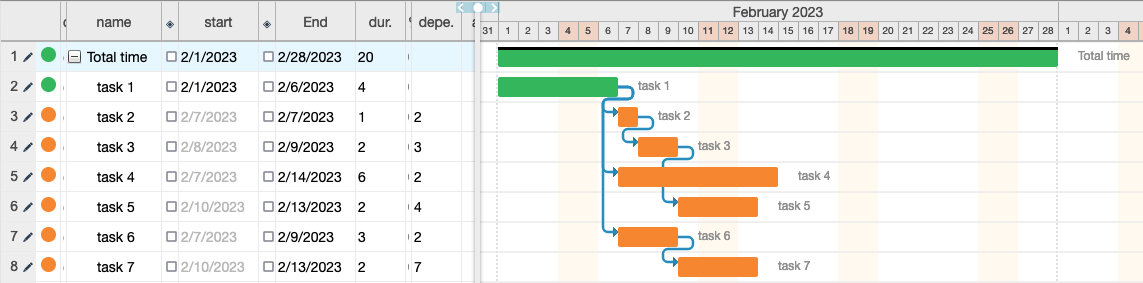
\includegraphics[scale = 0.4]{Figures/Gantt_1.png}

\subcaption{Precedences of the source input}

\vspace{0.2cm}

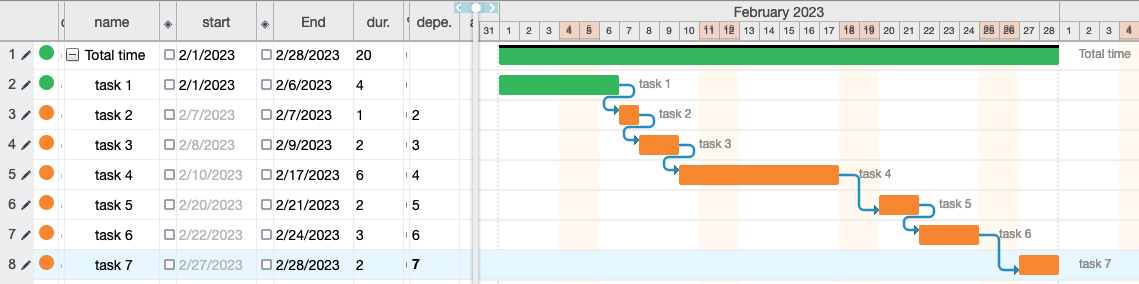
\includegraphics[scale = 0.4]{Figures/Gantt_2.png}

\subcaption{Precedences of the source input}
\end{center}
\caption{State of the precedence in the source and follow-up inputs of the MR1}
\label{Fig:Gantts}
\end{figure*}
\end{comment}



\section{Metamorphic Relations}\label{sec:metamorfic_relations}


This section exposes the MRs that we propose to detect possible errors
related to modeling scheduling problems: specifically, errors
that are located in precedence and resource sharing
constraints. Each MR is a condition $MR$ that depends
on 4 elements: $i_{1}$ a scheduling problem instance, $i_{2}$ the
following-up scheduling instance that is obtained by modifying
$i_{1}$, $o_{1}$ the output corresponding to $i_{1}$, and $o_{2}$ the
following-up output that is the output of $i_{2}$. A valid
implementation, a model in our case, should make true the MR.

% Figures used in this section (i.e. Figure \ref{Fig:Gantts}) has been created with the Twproject Gantt editor\footnote{https://gantt.twproject.com/}  that allows us to create projects, but not relies on a constraint solver.

%The first two MRs, shown below, are related to precedence constraints.


\subsection{MR1. Sequentially of all tasks}


% Si es satisfactible y se establecen precedencias de tal forma que todas las tareas se ejecutan en orden secuencial $\rightarrow$ el resultado tiene que ser satisfactible.

Let us consider a scheduling problem instance $i_1 = (T, P, D, \prec, R,
L, \dln)$ such than $|P|=1$ and $\dln\geq\sum_{i=1}^{n}D(t_{i},p_{1})$.
Then we build the scheduling instance problem
$mr_{1}(i_{1})=(T, D, \prec_{2}, R, L, \dln)$ build as follows. Let us
consider $i_{2}=m(i_{1})$, $o_{1}=\sol(i_{1})$, and
$o_{2}=\sol(i_{2})$.
Then, we define $t_{i}\prec_{2} t_{j}$ iff $i<j$, that is, we have a lineal
precedence relation. In these circumstances, if $i_{1}$ has a
solution, that is $o_{2}<\infty$,
then $i_{2}$ has a solution $o_{2}$ such that
$o_{2}\leq\sum_{i=1}^{|T|}D(t_{i})$.

\begin{framed}
  \begin{displaymath}
      \begin{array}{l}
        MR_{1}(i_1,i_2,o_{1},o_{2}):\\
        \hskip 1em i_1=(T,D,\prec,R,L,\dln)\wedge  \\
        \hskip 1em i_2=mr_1(i_1)\wedge o_{1}=\sol(i_{1})\wedge o_{2}=\sol(i_2)\\
      \hskip 1em \wedge o_{1}<\infty\wedge \dln>=\sum_{i=1}^{|T|}D(T(i)) \\
      \hskip 1em \longrightarrow o_2\leq \sum_{i=1}^{|T|}D(T(i))
    \end{array}
  \end{displaymath}
\end{framed}

% \begin{comment}

% \begin{figure}[!h]
% \begin{framed}

% \begin{center}
% \begin{tikzpicture}

%  \node [mynode](1) at (-3,0) {$t_1$};
%  \node [mynode](2) at (-1.5,1) {$t_2$};
%  \node [mynode](3) at (-1.5,-1) {$t_3$};
%  \node [mynode](4) at (0,0) {$t_4$};
%  \node [mynode](5) at (1.5,1) {$t_5$};

%  \draw[myarrow](1) -- (2);
%  \draw[myarrow](2) -- (3);
%  \draw[myarrow](3) -- (4);
%  \draw[myarrow](4) -- (5);
%  \draw[myarrow](2) -- (5);
% \end{tikzpicture}
% \subcaption{Precedences of the source input}

% \vspace{0.5cm}

% \begin{tikzpicture}
%  \node [mynode](1) at (-3,0) {$t_1$};
%  \node [mynode](2) at (-1.5,0) {$t_2$};
%  \node [mynode](3) at (0,0) {$t_3$};
%  \node [mynode](4) at (1.5,0) {$t_4$};
%  \node [mynode](5) at (3,0) {$t_5$};

%  \draw[myarrow](1) -- (2);
%  \draw[myarrow](2) -- (3);
%  \draw[myarrow](3) -- (4);
%  \draw[myarrow](4) -- (5);
% \end{tikzpicture}
% \subcaption{Precedences of the source input}
% \end{center}
% \end{framed}
% \caption{State of the precedences in the source and follow-up inputs of the MR1}
% \label{Fig:MR1-Sequentility-all-tasks}
% \end{figure}

% \end{comment}

% https://gantt.twproject.com:443/project/3KI-D240DD9B1E7477F7D928FC021F21670D13BC5B50403445C9FCA48EBBE477BEB0
















\subsection{MR2. Add inverse precedence}
The idea of this MR is that if we introduce a dependency that
introduce a cycle in a scheduling problem instance with a solution,
then the new problem has no solutions. Formally,
let us consider $i_{1}=(T, P, D, \prec, R, L, \dln)$,
$t_{i}, t_{j}\in T$ such that $t_{i}\prec t_{j}$, and
$o_{1}=\sol(i_{1})<\infty$.
Now let us consider
the modified instance problem as $mr_{2}(i_{1},)=(T, D, \prec_{2}, R, L,
\dln)$,
were $\prec_{2}$ is $\prec$ where the relation $t_{j}\prec t_{i}$ is
added, that is $\prec_{2}= (\prec_{1}\cup \{(t_{j}, t_{i})\})^{+}$.
If we take $i_{2}=mr_{2}(i_{1})$ and $o_{2}=\sol(i_{2})$, then
$o_{2}=\infty$.

\begin{framed}
  \begin{displaymath}
      \begin{array}{l}
    MR_{2}(i_1,i_2,o_{1},o_{2}):\\
      \hskip 1em i_1=(T,P,D,\prec,R,L,\dln)\wedge  \\
      \hskip 1em  i_2=mr_2(i_1)\wedge o_{1}=\sol(i_{1})\wedge o_{2}=\sol(i_2)\\
      \hskip 1em \wedge o_{1}<\infty
      \longrightarrow o_2=\infty
    \end{array}
  \end{displaymath}
\end{framed}


% \begin{framed}
% \textbf{MR2. Add inverse precedence}

% %Change forall to exists
% Si es satisfactible y se añade una precedencia que es la inversa de una que ya existe (forma un cliclo) $\rightarrow$ es insatisfactible.
% \end{framed}

% \begin{framed}
% \begin{center}
% $MR2(i_1,i_2,o_1,o_2)$

% $ \Updownarrow_{def}$

% $Sat (O_1)) \wedge pre = pre \texttt{++} [pre[1,2], pre[1,1]]$

% $\Downarrow$

% $Insat(O_2)$
% \end{center}
% \end{framed}



% Si se añade una precedencia que es la inversa de una que ya existe entonces quiere decir que hay un ciclo. Pero, si al añadir esa precedencia inversa sigue dando solución y no es insat, entonces quiere decir que se ha puesto un exists en vez de un forall.

% Obser: El que es insatisfactible tiene un forall y el que tiene solución tiene un exists es el programa mutado (basic-MUT-forall-exists.mzn)
% En este caso, no se ha encontrado un operador definido para este cambio de cuantificadores
% Podemos definirlo, indicando que se cambia un cuantificador lógico por otro (Existencial por universal o viceversa) .


% Esto se hace para matar al mutante que cambia forall por exists.



% Ejemplo correspondiente con el código de la carpeta MR2 del GitHUB y a la Figura \ref{Fig:MR2_Add-inverse-precedence}






% Original: constraint forall(i in PREC)

% Cambiado: constraint exists(i in PREC)

% En los datos se añade la precedencia  SOLDIERS $\rightarrow$ FUNDS para que forme  ciclo con la precedencia que ya existe que es
%  FUNDS $\rightarrow$ SOLDIERS









\subsection{MR3. Extreme duration}
The idea of this rule is that if we modify the duration long enough,
the whole scheduling will take longer. Let us consider
$i_{1}=(T, P, D, \prec, R, L, \dln)$, and sum of the duration
of all tasks in all processors and take an upper bound of this sum
$c>\sum_{i=1}^{|T|}\sum_{j=1}^{|P|}D(t_{i},p_{j})$. We modify the
duration of the task $1$ such that its duration is $D(1)+c$, formally, we
define
\begin{displaymath}
  D_{2}(t_{i}, p_{j})=
  \begin{cases}
    D(t_{1}, p_{1}) + c & \text{if } i=1, j=1\\
    D(t_{i}, p_{j}) & \text{otherwise}
  \end{cases}
\end{displaymath}
We take $\dln_{2}=\sum_{i=1}^{|T|}\sum_{j=1}^{|P|}D_{2}(t_{i},p_{j})$.
Then we take $mr_{3}(i_{1})=(T, D_{2}, \prec, R, L, \dln_{2})$. Let us
consider $o_{1}=\sol(i_{1})$, $i_{2}=mr_{3}(i_{1})$ and
$o_{2}=\sol(i_{2})$.
If $o_{1}\infty$ then $o_{1}<o_{2}<\infty$.

\begin{framed}
  \begin{displaymath}
      \begin{array}{l}
    MR_{3}(i_1,i_2,o_{1},o_{2}):\\
      \hskip 1em i_1=(T,P,D,\prec,R,L,\dln) \wedge  \\
      \hskip 1em  i_2=mr_3(i_1)\wedge o_{1}=\sol(i_{1})\wedge o_{2}=\sol(i_2)\\
      \hskip 1em \wedge o_{1}<\infty
      \longrightarrow o_{1}<o_2<\infty
    \end{array}
  \end{displaymath}
\end{framed}


% Hacemos un mutante donde cambiamos un \texttt{forall} por \texttt{exists},

% \texttt{jobshopMUT-forall-exists-1.mzn}.

% En este caso se aplica el nuevo operador de mutación en el que cambiamos un cuantificador por otro
% y este cambio se puede hacer en otras partes del código dando lugar a nuevos mutantes.








% \begin{comment}
% \begin{figure*}[h]
% \begin{minipage}{0.49\linewidth}
% \begin{center}
% \begin{tikzpicture}

%  \node [mynode](I) at (-2,1) {I (jdata.dzn) };
%  \node [mynode](O) at (-2,-2) {O (end = 30)};
%  \node [mylabel](code) at (0,-1) {jobshop.mzn};
%  \node [mynode](I') at (2,1) {I' (jdata+d)};
%  \node [mynode](O') at (2,-2) {O' (end = 126)};

%  \draw[myarrow](I) -- (O);
%  \draw[myarrow](I') -- (O');

%  \node [mynode,below= -0.3cm of I] (Icaption) {d[0,0] = 1};
%  \node [mynode,below= -0.3cm of I'] (I'caption) {d[0,0] = 100};

% \end{tikzpicture}
% \subcaption{MR execution}
% \end{center}
% \end{minipage}
% \begin{minipage}{0.49\linewidth}
% \begin{center}
% \begin{tikzpicture}

%  \node [mynode](I) at (-2,1) {I (jdata.dzn) };
%  \node [mynode](O) at (-2,-2) {O (end = 21)};
%  \node [mylabel](code) at (-1,-1) {\verb+jobshopMUT-forall-exists-2.mzn+};
%  \node [mynode](I') at (2,1) {I' (jdata+d)};
%  \node [mynodeRed](O') at (2,-2) {O' (end = 21)};

%  \draw[myarrow](I) -- (O);
%  \draw[myarrow](I') -- (O');

%  \node [mynode,below= -0.3cm of I] (Icaption) {d[0,0] = 1};
%  \node [mynode,below= -0.3cm of I'] (I'caption) {d[0,0] = 100};

% \end{tikzpicture}
% \subcaption{Mutation execution}
% \end{center}
% \end{minipage}
% \caption{MR3. Caso 2 de cambio forall - exists en el código de jobshop}
% \label{Fig:jobshop-forall-exists-2}
% \end{figure*}
% \end{comment}









% La Metamorphic Relation \texttt{Extreme Durations}, también mata a otro mutante.

% \texttt{jobshopMUT-and-or.mzn}

% En este caso se ha cambiado la conjunción por la disyunción: \verb+/\  -> \/+

% \begin{comment}
% \begin{figure*}[h]
% \begin{minipage}{0.49\linewidth}
% \begin{center}
% \begin{tikzpicture}

%  \node [mynode](I) at (-2,1) {I (jdata.dzn) };
%  \node [mynode](O) at (-2,-2) {O (end = 30)};
%  \node [mylabel](code) at (0,-1) {jobshop.mzn};
%  \node [mynode](I') at (2,1) {I' (jdata+d)};
%  \node [mynode](O') at (2,-2) {O' (end = 126)};

%  \draw[myarrow](I) -- (O);
%  \draw[myarrow](I') -- (O');

%  \node [mynode,below= -0.3cm of I] (Icaption) {d[0,0] = 1};
%  \node [mynode,below= -0.3cm of I'] (I'caption) {d[0,0] = 100};

% \end{tikzpicture}
% \subcaption{MR execution}
% \end{center}
% \end{minipage}
% \begin{minipage}{0.49\linewidth}
% \begin{center}
% \begin{tikzpicture}

%  \node [mynode](I) at (-2,1) {I (jdata.dzn) };
%  \node [mynode](O) at (-2,-2) {O (end = 0)};
%  \node [mylabel](code) at (-0.7,-1) {jobshopMUT-and-or.mzn};
%  \node [mynode](I') at (2,1) {I' (jdata+d)};
%  \node [mynodeRed](O') at (2,-2) {O' (end = 0)};

%  \draw[myarrow](I) -- (O);
%  \draw[myarrow](I') -- (O');

%  \node [mynode,below= -0.3cm of I] (Icaption) {d[0,0] = 1};
%  \node [mynode,below= -0.3cm of I'] (I'caption) {d[0,0] = 100};

% \end{tikzpicture}
% \subcaption{Mutation execution}
% \end{center}
% \end{minipage}
% \caption{MR3. jobshop cambiar y por o}
% \label{Fig:jobshop-y-o}
% \end{figure*}
% \end{comment}




% \subsection{cumulative constraint (resources)}


% The cumulative constraint is used for describing cumulative resource usage.

% \texttt{cumulative(array[int] of var int: s, array[int] of var int: d, array[int] of var int: r, var int: b)}

% Schedule for moving furniture:
% It requires that a set of tasks given by start times $s$, durations $d$, and resource requirements $r$, never require more than a global resource bound $b$ at any one time.

% Los códigos son \texttt{Codes/moving.mzn} y \texttt{Codes/moving.dzn}.







\subsection{MR4. More resources}
This rule establishes that if we take more resources, the
time required to complete all tasks is, at most, the original one.
Let us consider
$i_{1}=(T, P, D, \prec, R, L, \dln)$, for each $r\in R$ we take a
positive integer $c_{r}$ and then we define
\begin{displaymath}
  R_{2}(r)=R(r)+c_{r}\quad \forall r\in R
\end{displaymath}
Then we take $mr_{4}(i_{1}) = (T, D, \prec, R_{2}, L, \dln)$.
Let us
consider $o_{1}=\sol(i_{1})$, $i_{2}=mr_{4}(i_{1})$ and
$o_{2}=\sol(i_{2})$.
If $o_{1}<\infty$ then $o_{2}\leq o_{1}$.

\begin{framed}
  \begin{displaymath}
      \begin{array}{l}
    MR_{4}(i_1,i_2,o_{1},o_{2}):\\
      \hskip 1em  i_1=(T,P,D,\prec,R,L,\dln) \wedge\\
      \hskip 1em  i_2=mr_3(i_1)\wedge o_{1}=\sol(i_{1})\wedge o_{2}=\sol(i_2)\\
      \hskip 1em \wedge o_{1}<\infty
      \longrightarrow o_{2}\leq o_1
    \end{array}
  \end{displaymath}
\end{framed}

%     Si es satisfactible y aumentamos los recursos  (handlers and trolleys) $\rightarrow$  el resultado tiene que ser satisfactible y el makespan (end) se reduce o se queda igual ($<=$).
% \end{framed}

% $ i_1 = (T1, D1, - , - , R1 , time1 )$

% $ i_2 = (T2, D2, - , - , R2 , time2 )$

% where
% $R1 = [(l1_1,up1_1), \dots, (l1_k,up1_k)]$

% $O_1 = S(i_1)$

% \begin{framed}
% \begin{center}
% $MR4(i_1,i_2,o_1,o_2)$

% $ \Updownarrow_{def}$

% $Sat (O_1)) \wedge$

% $\forall i \in \{1,\dots,k\} \ \exists j \in \{1,\dots,k\}$ and $\exists c >0$ \texttt{such as} $up2_j = up1_j + c $

% $\Downarrow$

% $Sat(O_2) \wedge  \texttt{makespan($O_2$)} =< \texttt{makespan($O_1$)} $
% \end{center}
% \end{framed}










% \begin{comment}

% \begin{framed}

% \textbf{MR5. Fewer resources}

% Si es satisfactible y disminuimos elos recursos  (handlers and trolleys)  $\rightarrow$  el resultado tiene que ser uno de estos dos casos:
% \begin{itemize}
%     \item Satisfactible y el makespan se amplía o se queda igual (\texttt{>=})
%     \item o es insatisfactible
%     %(porque no cumple  forall( r in RESOURCE, t in TASK) ( res[r,t]  $<=$ L[r])).
% \end{itemize}
% \end{framed}

% \begin{framed}
% \begin{center}
% $MR5(i_1,i_2,o_1,o_2)$

% $ \Updownarrow_{def}$

% $Sat (O_1)) \wedge$

% $\forall i \in \{1,\dots,k\} \ \exists j \in \{1,\dots,k\}$ and $\exists c >0$ \texttt{such as} $up2_j = up1_j - c $

% $\Downarrow$

% $(InSat(O_2)) \vee $

% $(Sat(O_2) \wedge \texttt{makespan($O_2$)} \geq \texttt{makespan($O_1$)}) $
% \end{center}
% \end{framed}
% \end{comment}




% \begin{comment}

% \begin{figure*}[h]
% \begin{minipage}{0.49\linewidth}
% \begin{center}
% \begin{tikzpicture}

%  \node [mynode](I) at (-1.5,1) {I (cumul-sched.dzn) };
%  \node [mynode](O) at (-1.5,-2) {O (end = 90)};
%  \node [mylabel](code) at (0,-1) {cumul-sched.mzn};
%  \node [mynode](I') at (1.5,1) {I' (cumul-sched-fu.dzn)};
%  \node [mynode](O') at (1.5,-2) {O' (end = 120)};

%  \draw[myarrow](I) -- (O);
%  \draw[myarrow](I') -- (O');

%  \node [mynode,below= -0.3cm of I] (Icaption) {[4,4,4]};
%  \node [mynode,below= -0.3cm of I'] (I'caption) {[3,3,2]};

% \end{tikzpicture}
% \subcaption{MR execution}
% \end{center}
% \end{minipage}
% \begin{minipage}{0.49\linewidth}
% \begin{center}

% \begin{tikzpicture}
%  \node [mynode](I) at (-1.5,1) {I (cumul-sched.dzn)};
%  \node [mynode](O) at (-1.5,-2) {O (end = 85)};
%  \node [mylabel](code) at (0,-1) {cumul-MUT-forall-notforall.mzn};
%  \node [mynode](I') at (1.5,1) {I' (85)};
%  \node [mynode](O') at (1.5,-2) {O' (85)};

%  \draw[myarrow](I) -- (O);
%  \draw[myarrow](I') -- (O');

%  \node [mynode,below= -0.3cm of I] (Icaption) {[4,4,4]};
%  \node [mynode,below= -0.3cm of I'] (I'caption) {[3,3,2]};

% % \draw[->,red, thick](T1) -- (T2);
% \end{tikzpicture}
% \subcaption{Mutation execution}
% \end{center}
% \end{minipage}
% \caption{MR5}
% \label{Fig:cumul-sched}
% \end{figure*}




% \begin{figure*}[h]
% \begin{minipage}{0.49\linewidth}
% \begin{center}
% \begin{tikzpicture}

%  \node [mynode](I) at (-1.5,1) {I (cumul-sched.dzn) };
%  \node [mynode](O) at (-1.5,-2) {O (end = 90)};
%  \node [mylabel](code) at (0,-1) {cumul-sched.mzn};
%  \node [mynode](I') at (1.5,1) {I' (cumul-sched-fu.dzn)};
%  \node [mynode](O') at (1.5,-2) {O' (end = 120)};

%  \draw[myarrow](I) -- (O);
%  \draw[myarrow](I') -- (O');

%  \node [mynode,below= -0.3cm of I] (Icaption) {[4,4,4]};
%  \node [mynode,below= -0.3cm of I'] (I'caption) {[3,3,2]};

% \end{tikzpicture}
% \subcaption{MR execution}
% \end{center}
% \end{minipage}
% \begin{minipage}{0.49\linewidth}
% \begin{center}

% \begin{tikzpicture}
%  \node [mynode](I) at (-1.5,1) {I (cumul-sched.dzn)};
%  \node [mynode](O) at (-1.5,-2) {O (end = 85)};
%  \node [mylabel](code) at (0,-1) {cumul-MUT-forall-exists.mzn};
%  \node [mynode](I') at (1.5,1) {I' (85)};
%  \node [mynodeGreen](O') at (1.5,-2) {O' (100)};

%  \draw[myarrow](I) -- (O);
%  \draw[myarrow](I') -- (O');

%  \node [mynode,below= -0.3cm of I] (Icaption) {[4,4,4]};
%  \node [mynode,below= -0.3cm of I'] (I'caption) {[3,3,2]};

% % \draw[->,red, thick](T1) -- (T2);
% \end{tikzpicture}
% \subcaption{Mutation execution}
% \end{center}
% \end{minipage}
% \caption{MR5}
% \label{Fig:cumul-sched-2}
% \end{figure*}
% \end{comment}


\section{Mutants}\label{sec:mutants}
In order to check the validity of the MRs, we are going
to use mutation testing technique. We are going to select known
solutions of the scheduling problems in MiniZinc, and we are going to
generate mutants from them. We are going to consider useful a
metamorphic relation $MR$ if any follow-up test case generated by it,
is able to kill a mutant, that is able to detect an error and the $MR$ 
is not met. In order to achieve this, we have to find
an input $i_{1}$, the output from the mutant $o_{1}$, a following-up input
$i_{2}$, and its output from the mutant $o_{2}$ such that invalidate
the condition in the metamorphic relation.
%% parsai2literature
\subsection{Mutation operators}
\label{s:mutOp}
Besides the typical mutation operators~\cite{parsai2literature} in other contexts such as
arithmetic mutation (change a sum by a product), we need to introduce
specific mutation operators like changing an existential quantifier by
a universal one. In this work, we have considered the following
mutation operators:


\begin{description}
    \item[MUT$\leq$] Changing the relational operator \lstinline|<| by  \lstinline|<=|.
      The application of this operator appears in the mutant
      \url{https://github.com/LuisLlana/metamorphic_testing_constrints/blob/main/MR%201/basic-MUT-%3C%3D-%3C.mzn}.
    \begin{framed}
\begin{lstlisting}[basicstyle=\ttfamily\fontsize{7}{9}\selectfont]
start[pre[i,1]] + duration[pre[i,1]] < start[pre[i,2]]
\end{lstlisting}
      \vskip -2em
      \centering$\Updownarrow$
\begin{lstlisting}[basicstyle=\ttfamily\fontsize{7}{9}\selectfont]
start[pre[i,1]] + duration[pre[i,1]] <= start[pre[i,2]]
\end{lstlisting}
    \end{framed}

  \item[MUT$\forall\exists$]  Changing universal and existential quantifiers.
      The application of this operator appears in the mutant
      \url{https://github.com/LuisLlana/metamorphic_testing_constrints/blob/main/MR%202/basic-MUT-forall-exists.mzn}.
    \begin{framed}
\begin{lstlisting}[basicstyle=\ttfamily\fontsize{7}{9}\selectfont]
constraint exists(i in PREC)
\end{lstlisting}
      \vskip -2em
      \centering$\Updownarrow$
\begin{lstlisting}[basicstyle=\ttfamily\fontsize{7}{9}\selectfont]
constraint forall(i in PREC)
\end{lstlisting}
    \end{framed}

    \item[MUT$\wedge\vee$] Changing disjunctions by conjunctions. The application of
      this operator appears in the mutant
      \url{https://github.com/LuisLlana/metamorphic_testing_constrints/blob/main/MR%203/jobshopMUT-and-or.mzn}.

    \begin{framed}
\begin{lstlisting}[basicstyle=\ttfamily\fontsize{7}{9}\selectfont]
(s[i,j]+d[i,j]<=s[i,enum_next(TASK,j)]) \/
\end{lstlisting}
      \vskip -2em
      \centering$\Updownarrow$
\begin{lstlisting}[basicstyle=\ttfamily\fontsize{7}{9}\selectfont]
(s[i,j]+d[i,j]<=s[i,enum_next(TASK,j)]) /\
\end{lstlisting}
    \end{framed}
\begin{lstlisting}
\end{lstlisting}

\item[MUT$\Leftrightarrow$] Interchanging parameters in function calls. The application of
  this operator appear in the mutant
  \url{https://github.com/LuisLlana/metamorphic_testing_constrints/blob/main/MR%204/movingMUThandlers.mzn}.
    \begin{framed}
\begin{lstlisting}[basicstyle=\ttfamily\fontsize{7}{9}\selectfont,
  emph={handlers,duration}, emphstyle={\underbar}]
constraint cumulative(start, handlers, duration, available_handlers);
\end{lstlisting}
      \vskip -2em
      \centering$\Updownarrow$
\begin{lstlisting}[basicstyle=\ttfamily\fontsize{7}{9}\selectfont,
  emph={handlers,duration}, emphstyle={\underbar}]
constraint cumulative(start, duration, handlers, available_handlers);
\end{lstlisting}
    \end{framed}
From what we know, this mutation operator is new in mutation testing on declarative languages.
  \end{description}




%%% Local Variables:
%%% mode: latex
%%% TeX-master: "../MT_scheduling"
%%% End:
